% !TEX root = poster.tex
\node [mybox,anchor=north west, font=\fontsize{\fntszL}{\fntszL}\selectfont]
at (\appPos) (boxApp){%
\begin{minipage}{\bxszC}



% \begin{table}[h!]
%    %  \begin{center}
%      \begin{tabular}{cc}
% \includegraphics[clip,trim=0 0 0 0,width=0.36\textwidth]{figs/{ACME_Logo}.eps} &
% \begin{itemize}
% \item a
% \item a
% \end{itemize}
% \\
% second row &  \\
% and & so on \\
% \end{tabular}
%  %     \end{center}
%       \end{table}



      \begin{figure*}[ht]
 \subfloat{%
  \begin{tabular}{c}
\includegraphics[width=0.25\textwidth]{logos/{E3SM_Logo}.png}
  \end{tabular}
 }
 %
  \subfloat{%
  \fontsize{40}{40}\selectfont
  \begin{tabular}{p{28cm}}
  \begin{itemize}
     \item $\:$US Dep-t of Energy (DOE) Earth system model
 \item $\:$Land, atmosphere, ocean, ice, human system components; high-resolution
 \item $\:$ Employ DOE leadership computing facilities

\end{itemize}
  \end{tabular}
}
\end{figure*}
\vspace*{-1.cm}

%\includegraphics[width=0.97\textwidth,clip]{cmuq/{fit_LH_UMB_nm}.eps}
\includegraphics[width=0.97\textwidth,clip]{cmuq/{fit_LH_UMB_m}.eps}
%\includegraphics[width=0.97\textwidth,clip]{cmuq/{fit_NPP_UMB_nm}.eps}
\includegraphics[width=0.97\textwidth,clip]{cmuq/{fit_NPP_UMB_m}.eps}
%\includegraphics[width=0.97\textwidth,clip]{cmuq/{fit_LH_Ton_nm}.eps}
\includegraphics[width=0.97\textwidth,clip]{cmuq/{fit_LH_Ton_m}.eps}

\bigskip
\bigskip
\bigskip
\hrule
\hrule
\bigskip




\begin{figure*}[ht]
 \subfloat{%
  \begin{tabular}{c}
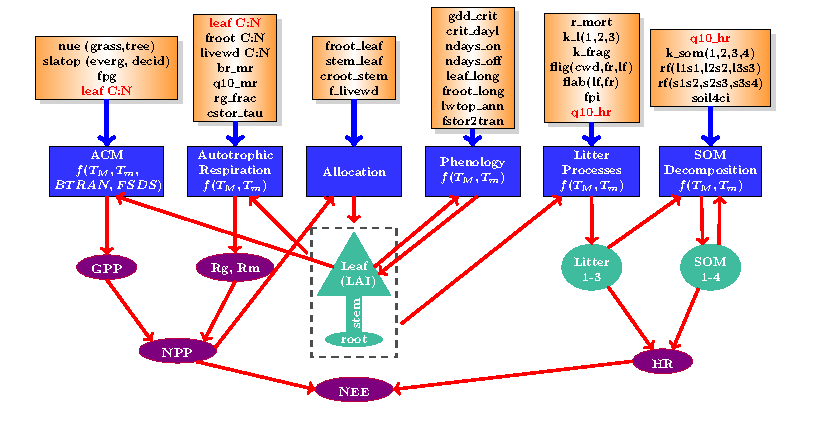
\includegraphics[width=0.52\textwidth]{figs_local/sketch.pdf}
  \end{tabular}
 }
 %
  \subfloat{%
  \fontsize{40}{40}\selectfont
  \begin{tabular}{p{17cm}}
  \begin{itemize}
     \item \textbf{ELM-LF} is a lower-fidelity, python version of ELM.
     \item  Calibration with select FLUXNET sites data.
\item Model error is the dominant uncertainty component: removes biases and overfitting.
\end{itemize}
  \end{tabular}
}
\end{figure*}

\begin{center}
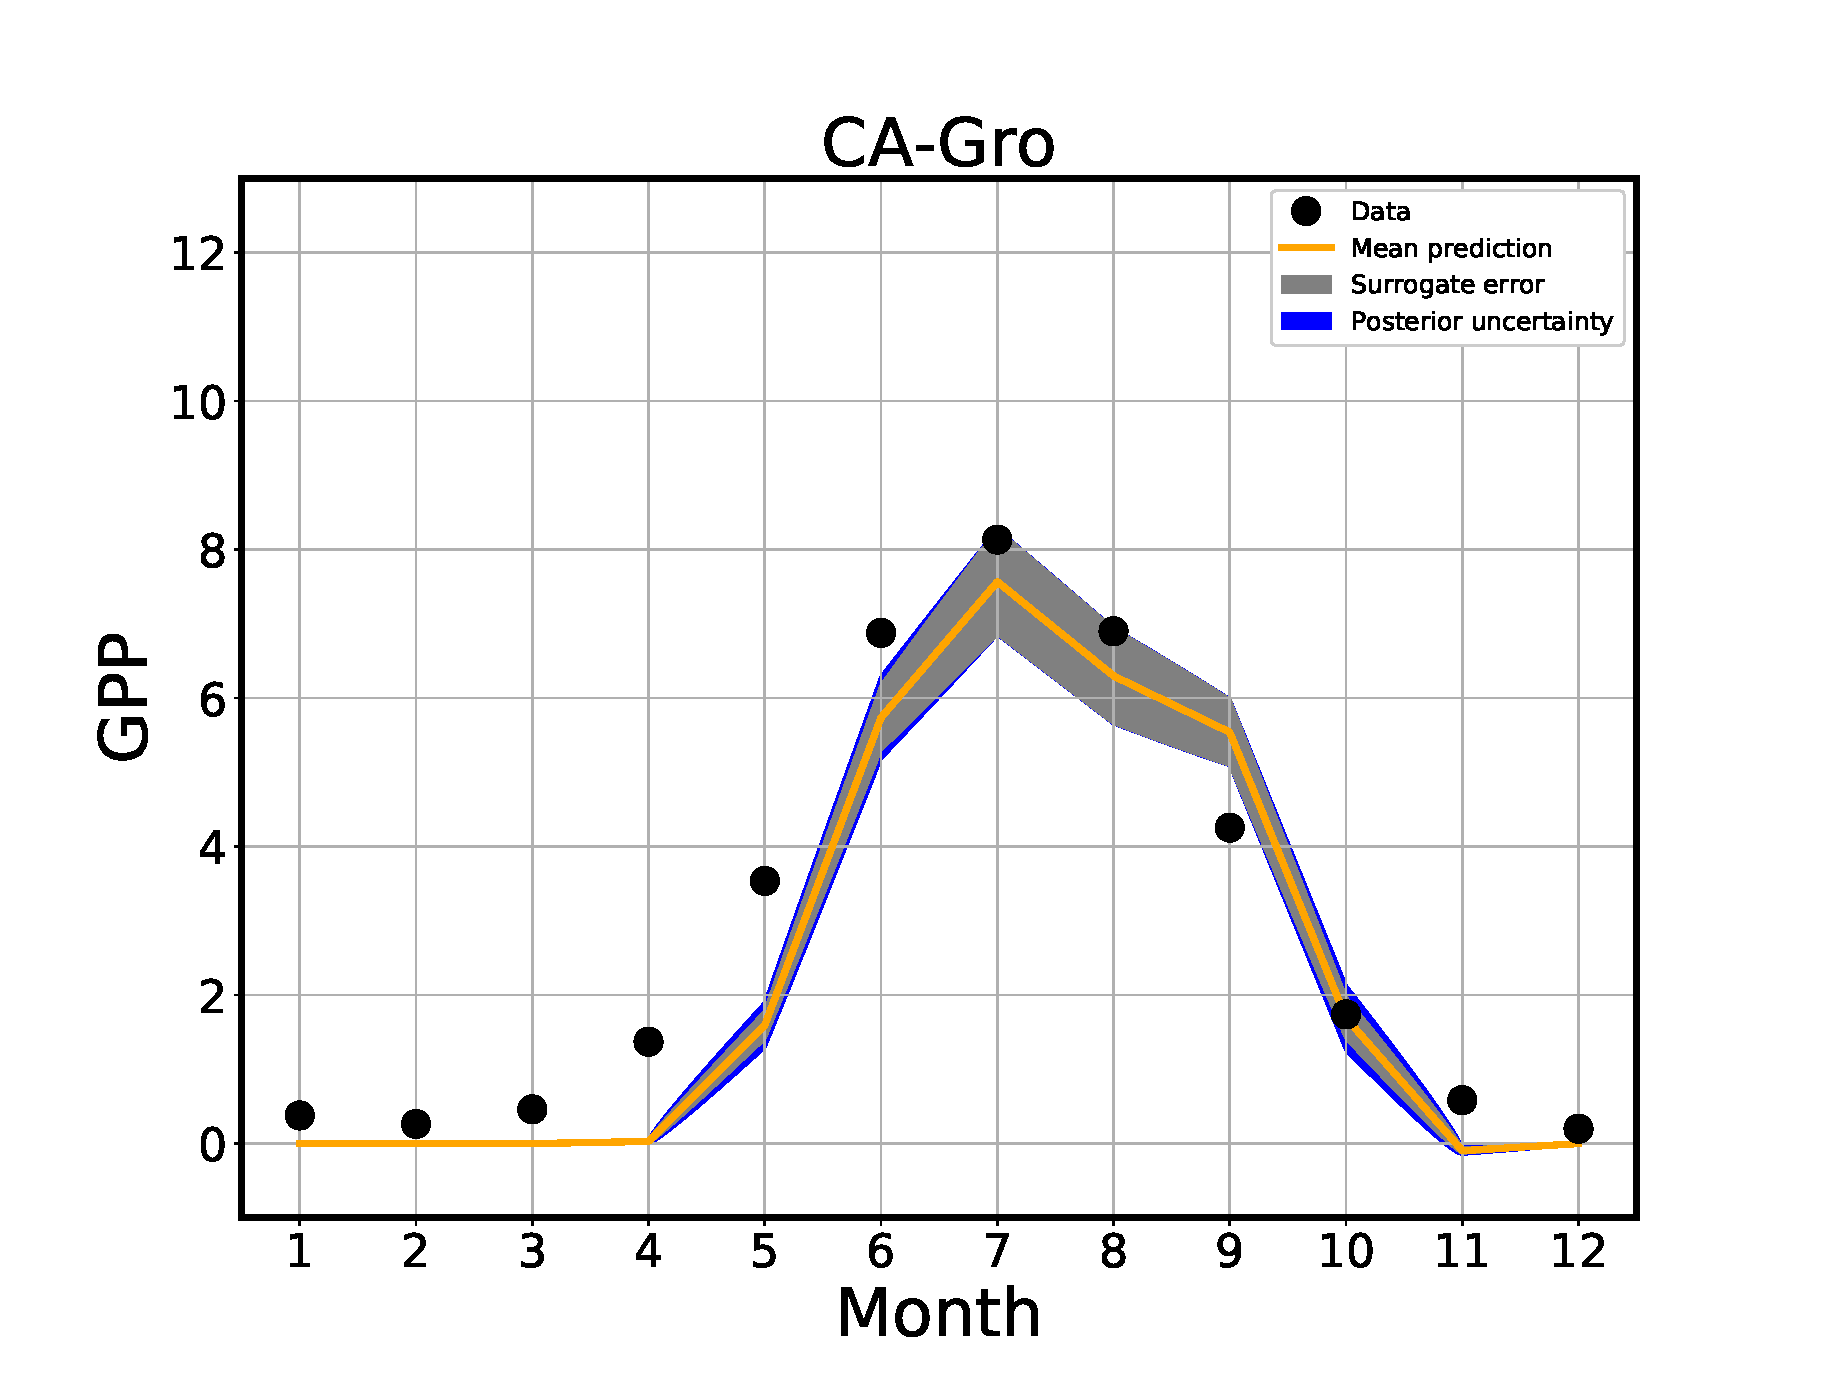
\includegraphics[width=0.24\textwidth]{figs_local/fit_CA-Gro.eps}
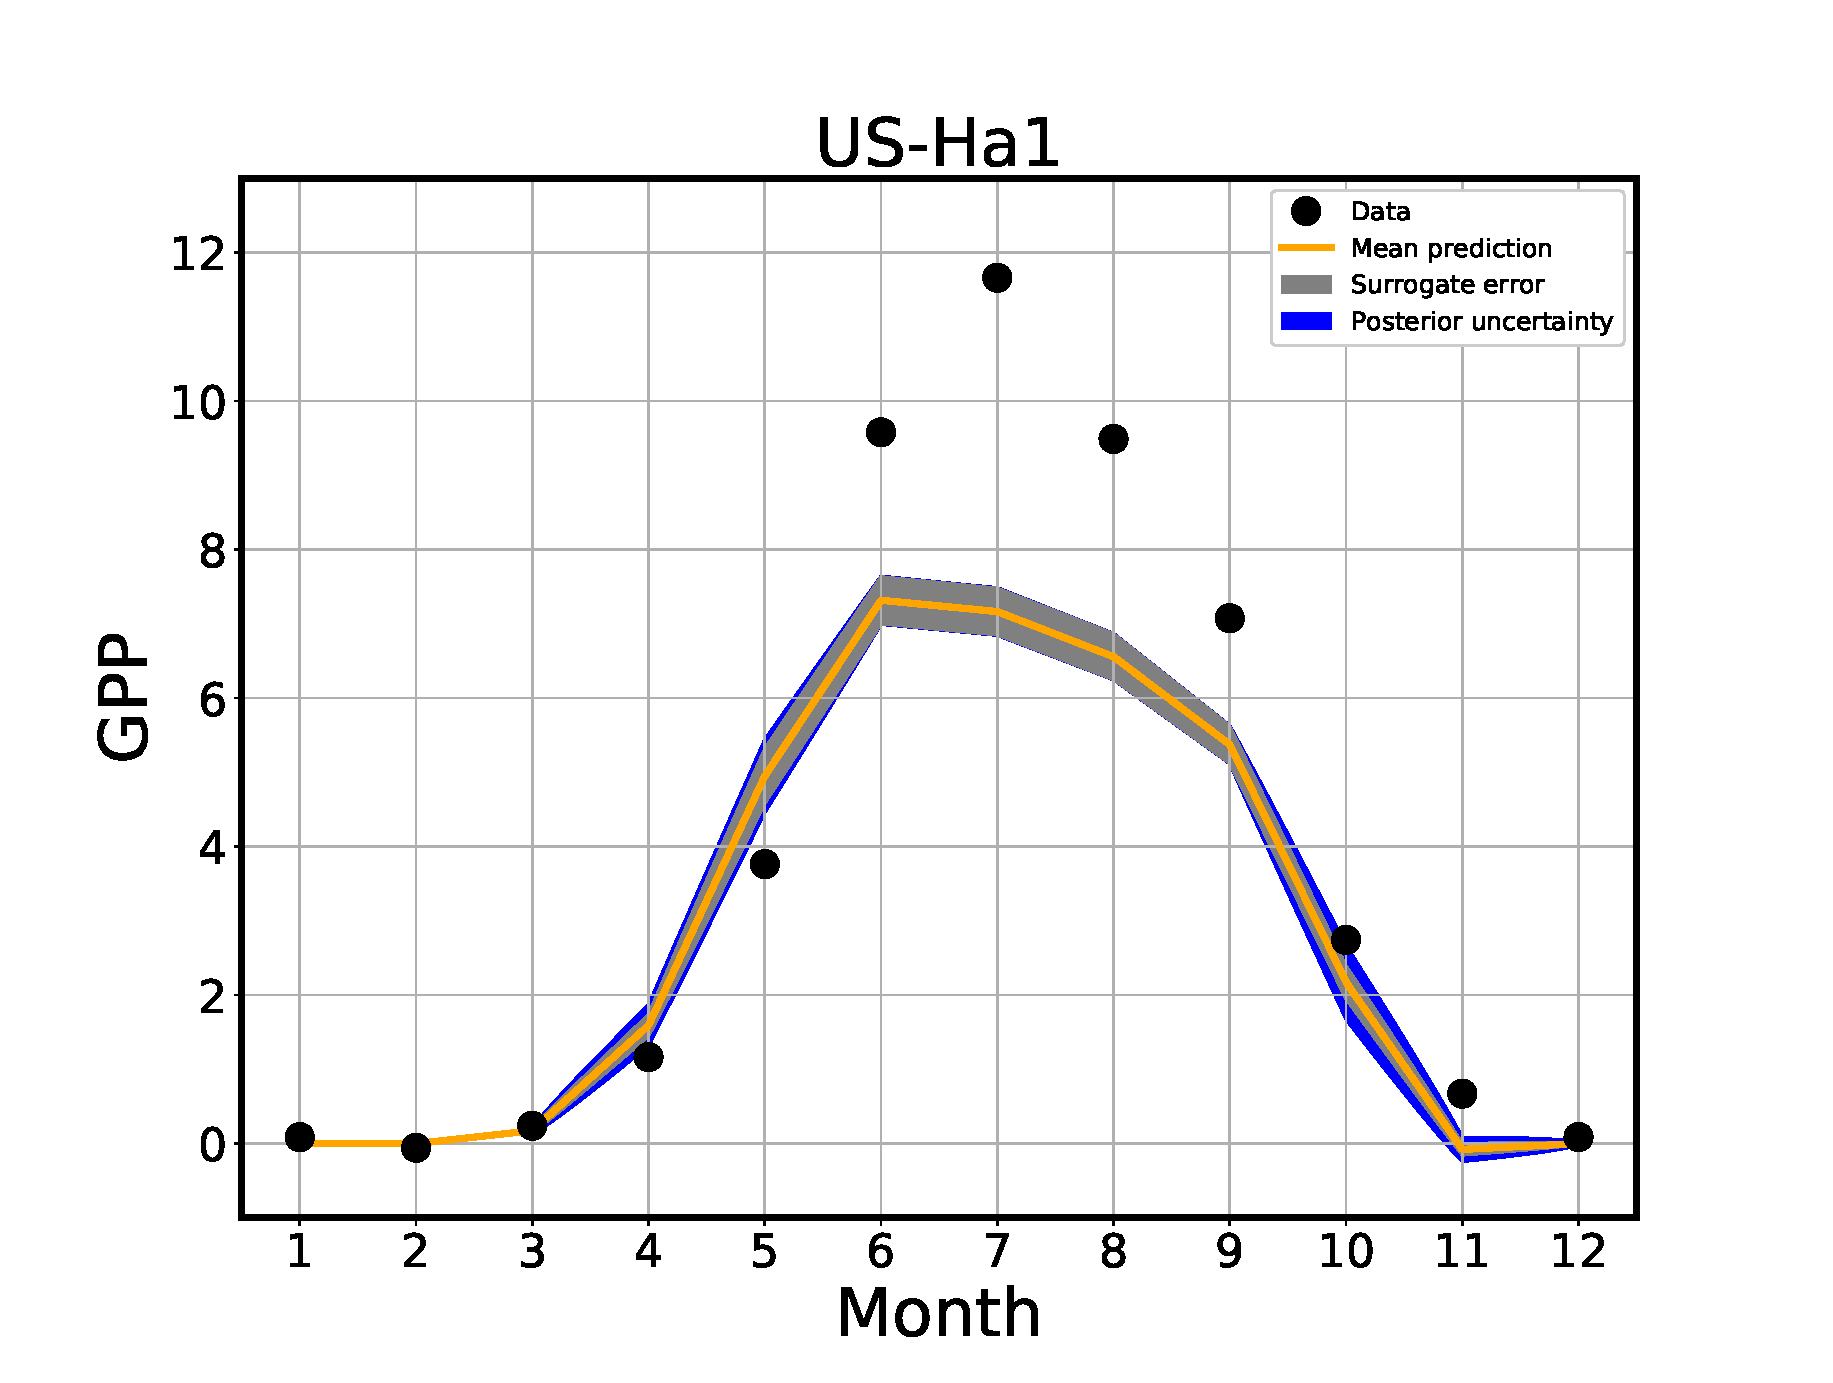
\includegraphics[width=0.24\textwidth]{figs_local/fit_US-Ha1.eps}
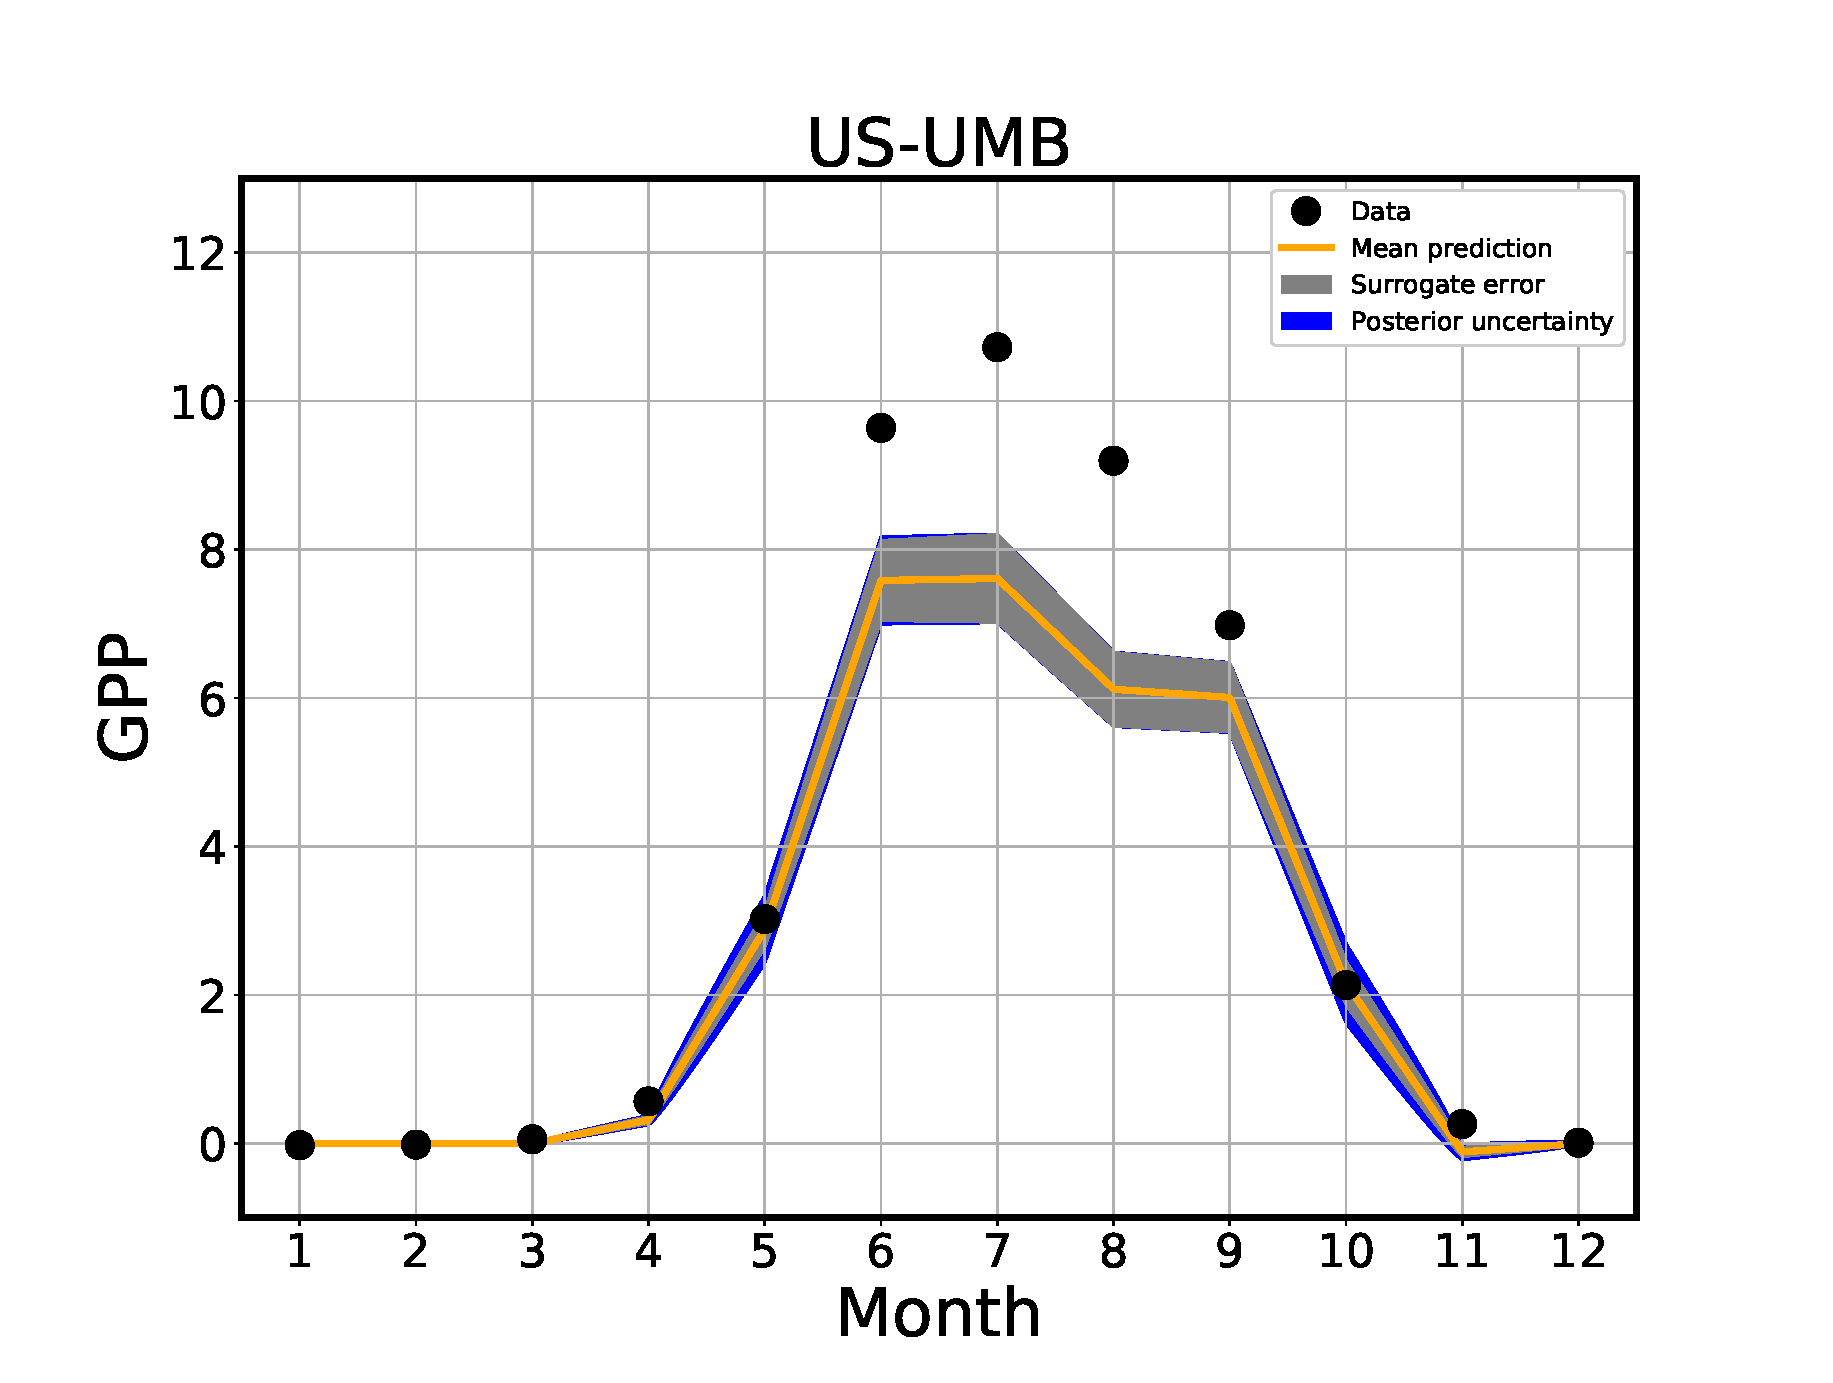
\includegraphics[width=0.24\textwidth]{figs_local/fit_US-UMB.eps}
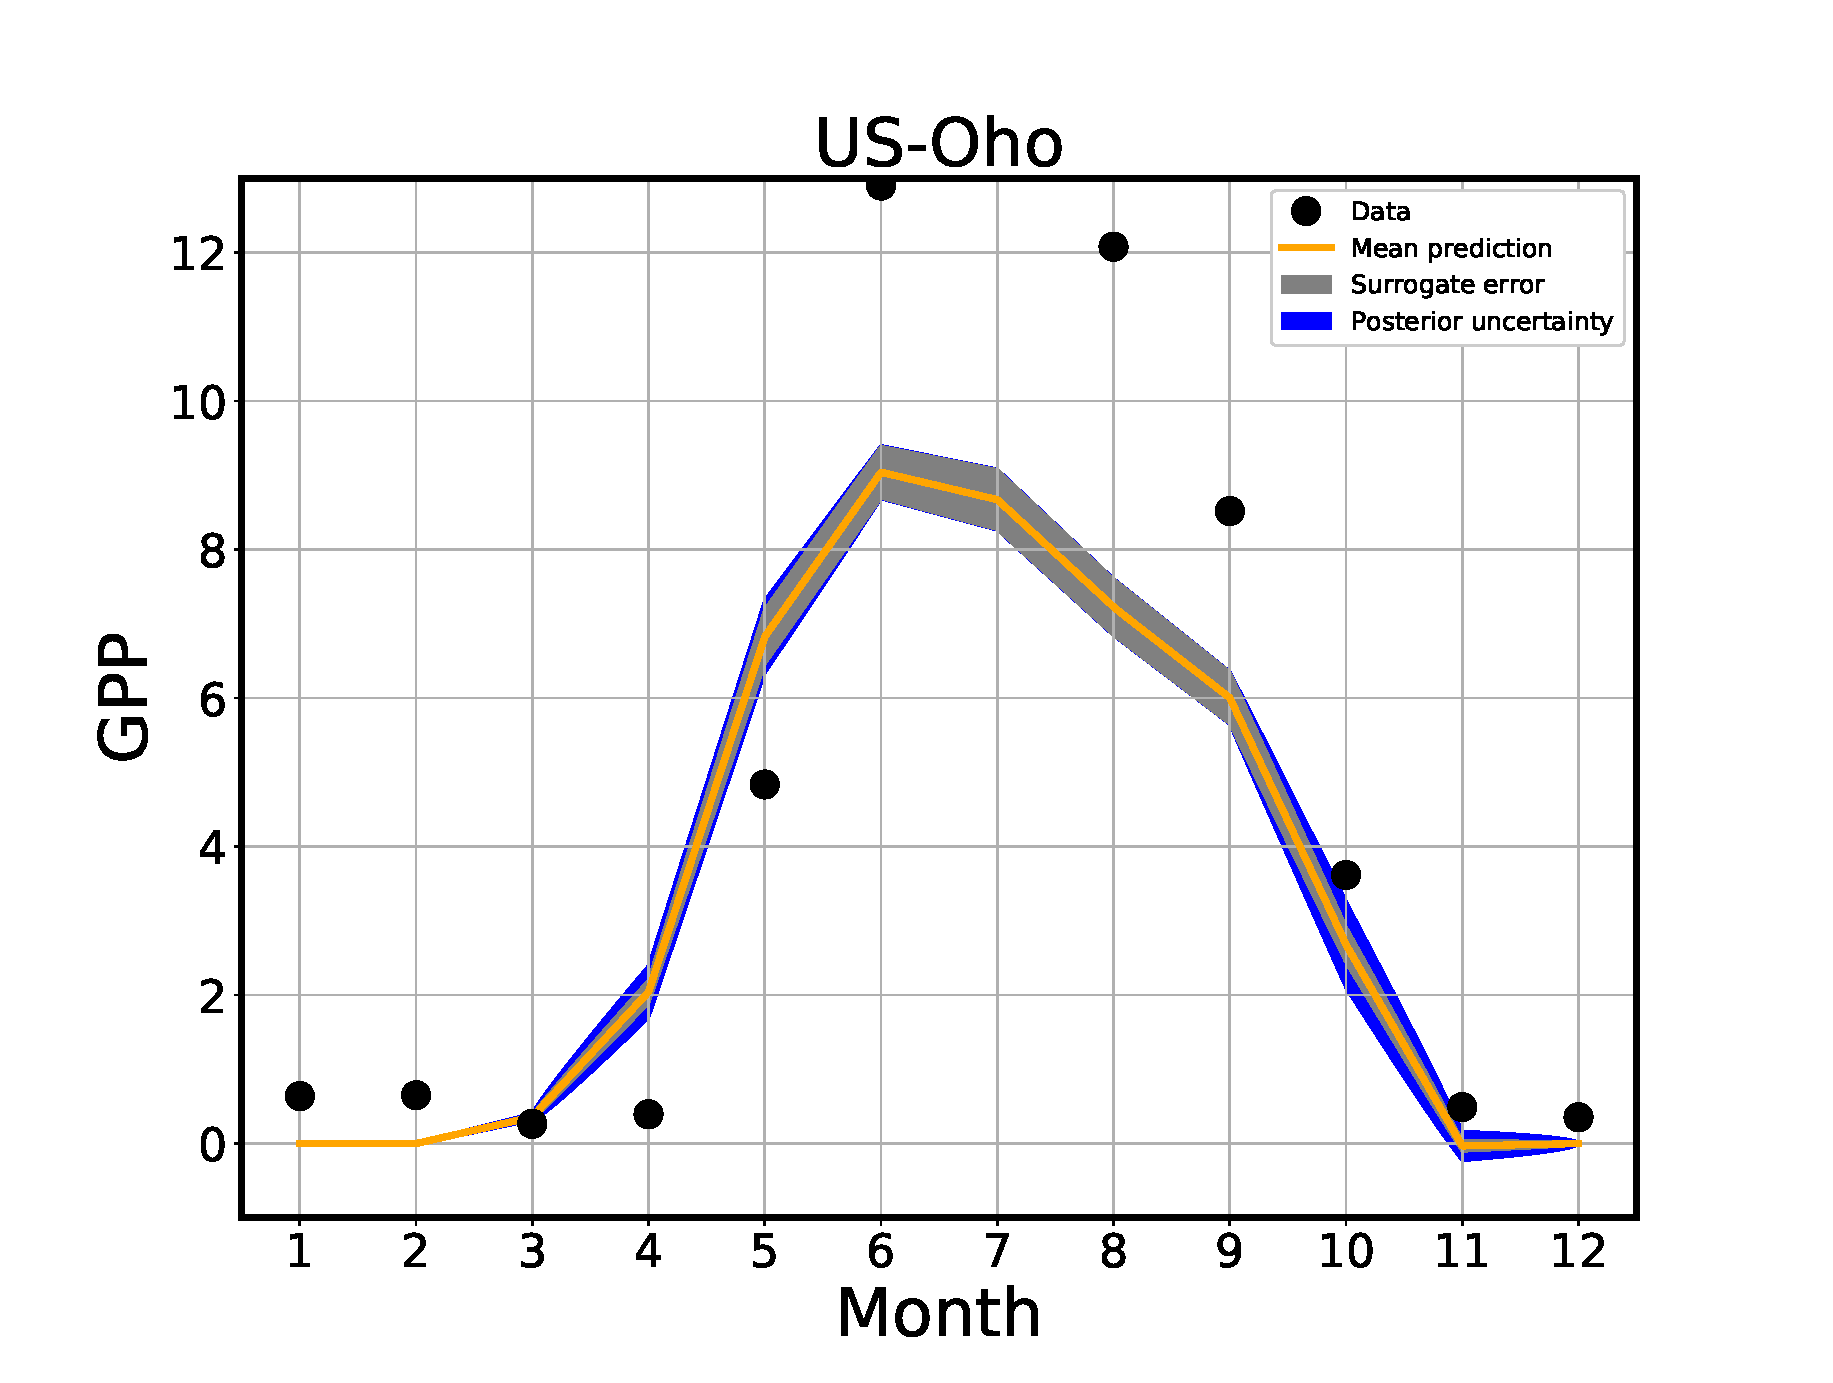
\includegraphics[width=0.24\textwidth]{figs_local/fit_US-Oho.eps}\\
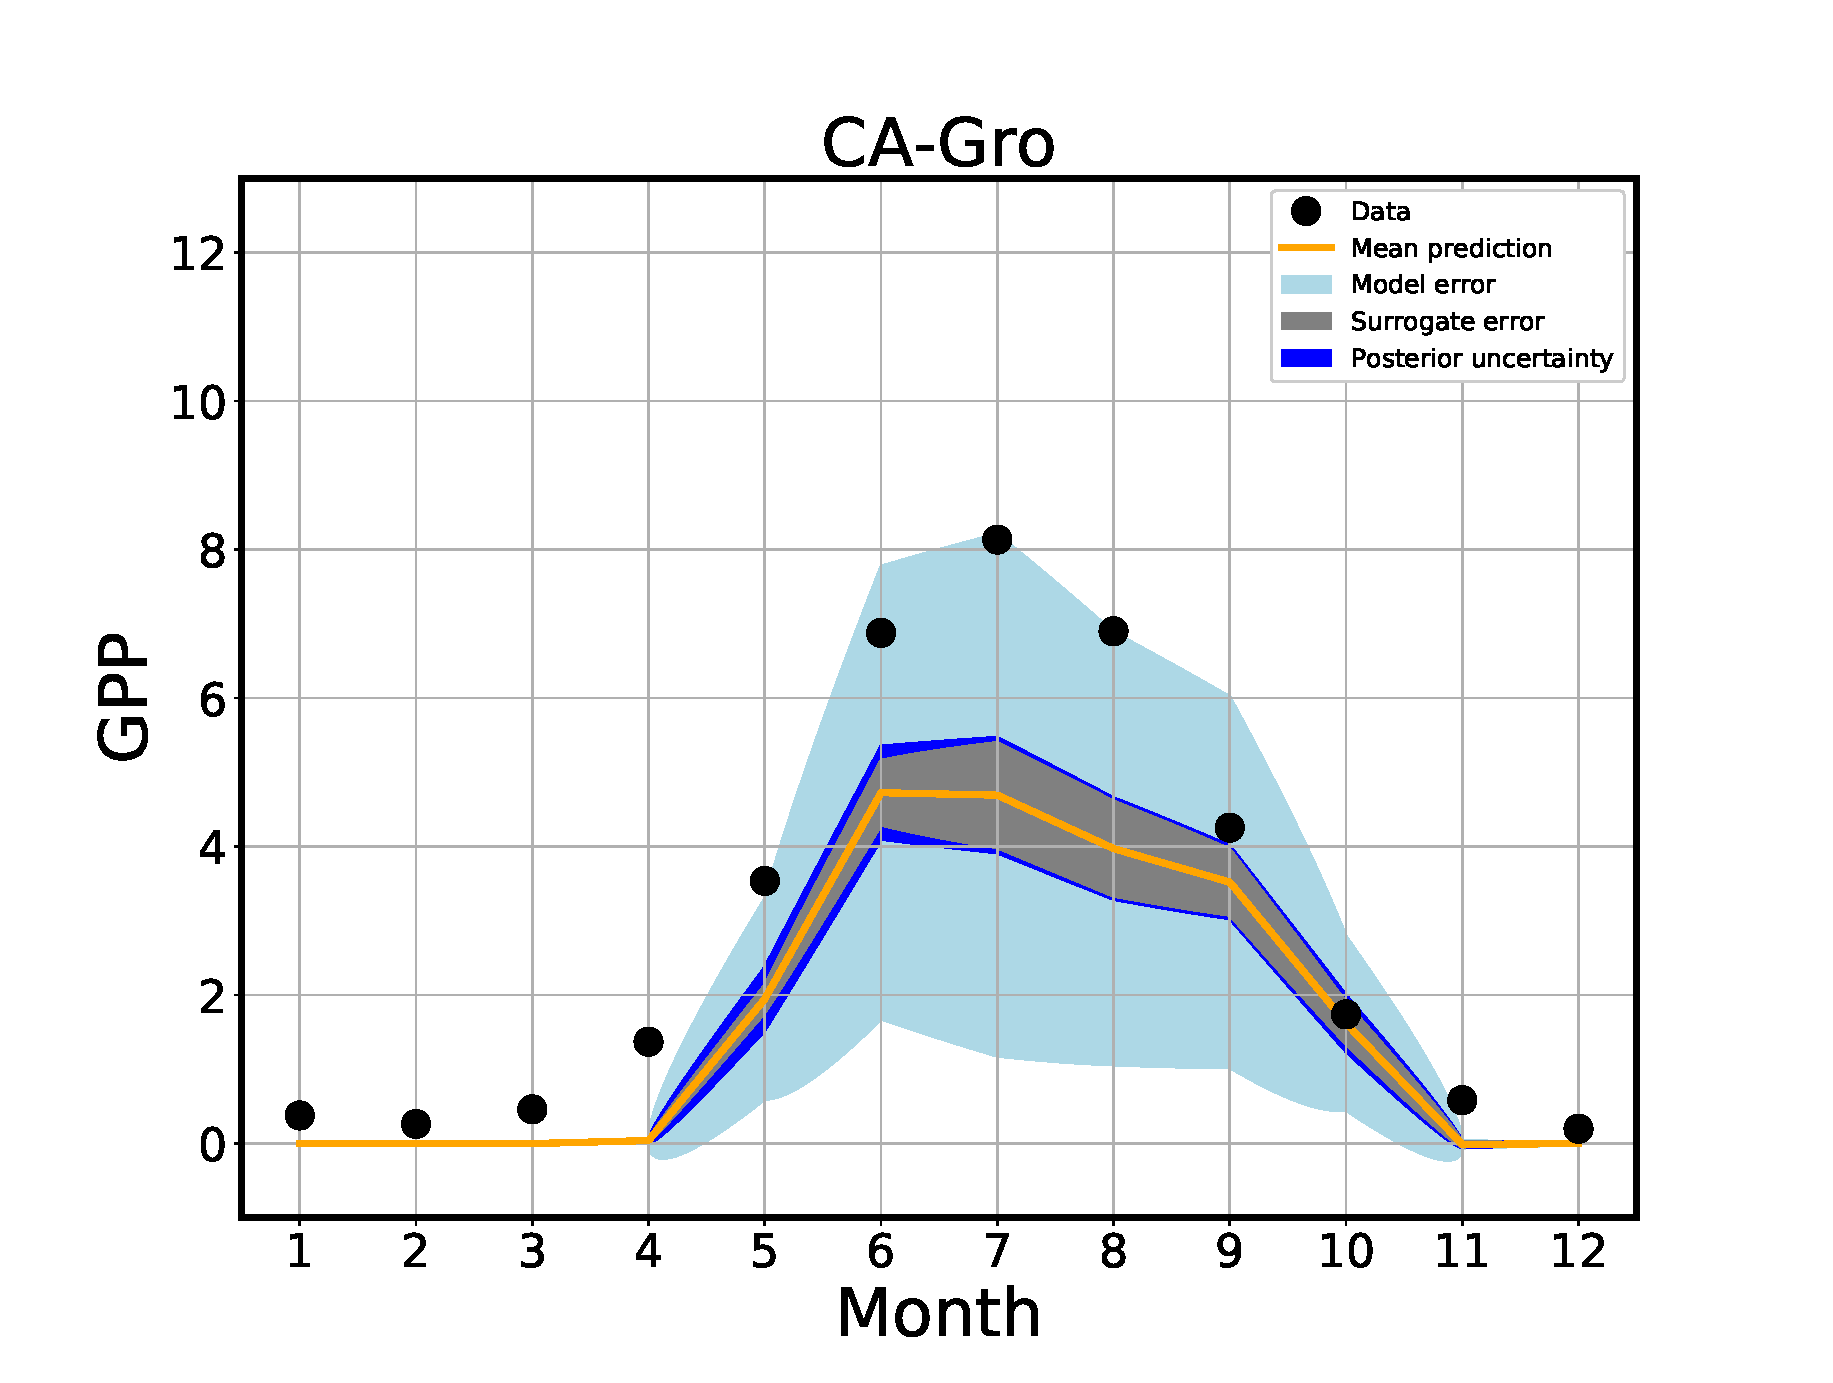
\includegraphics[width=0.24\textwidth]{figs_local/fit_CA-Gro_merr.eps}
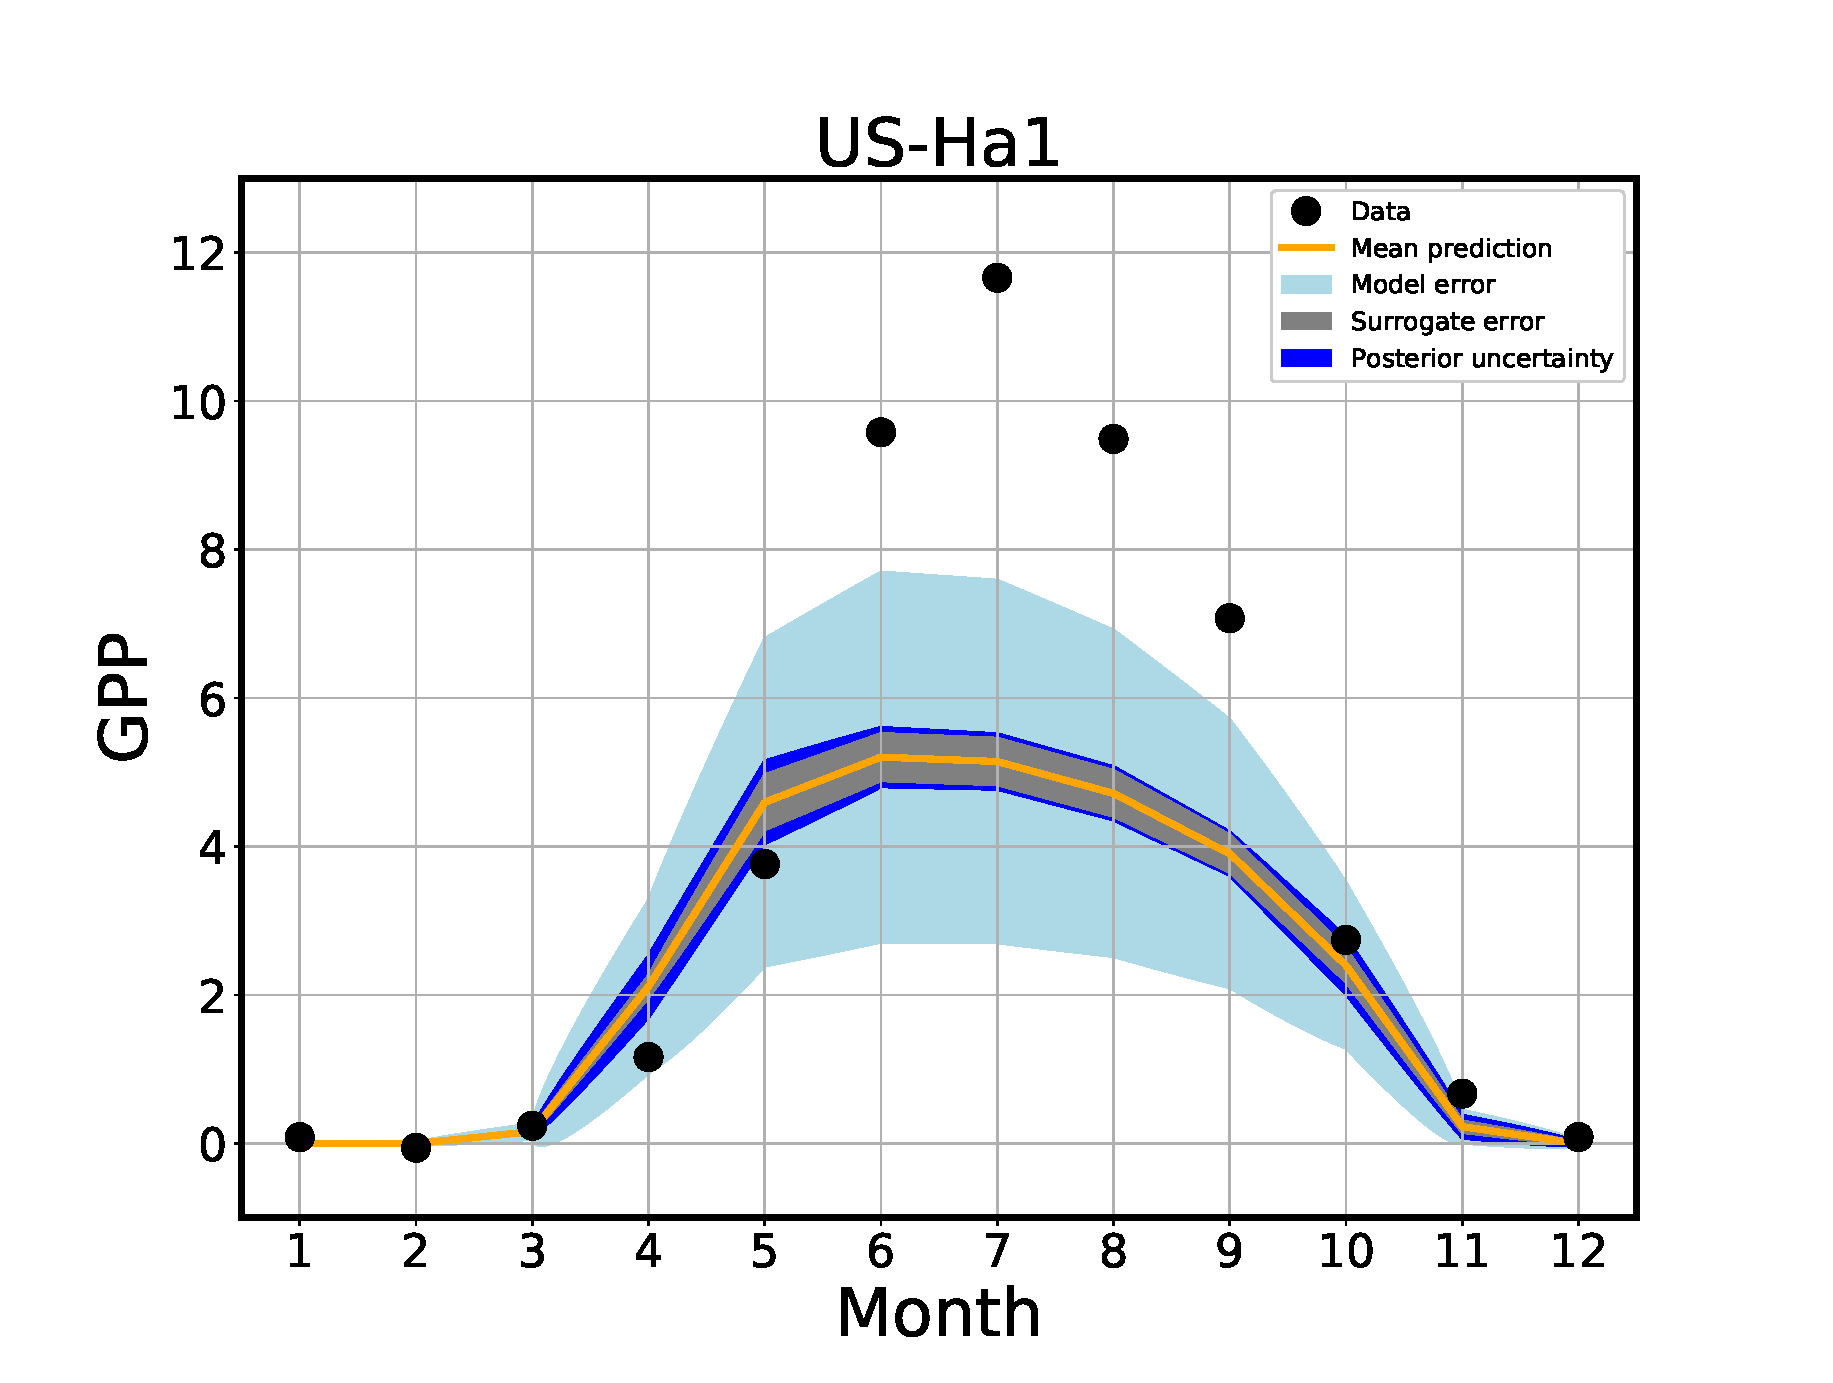
\includegraphics[width=0.24\textwidth]{figs_local/fit_US-Ha1_merr.eps}
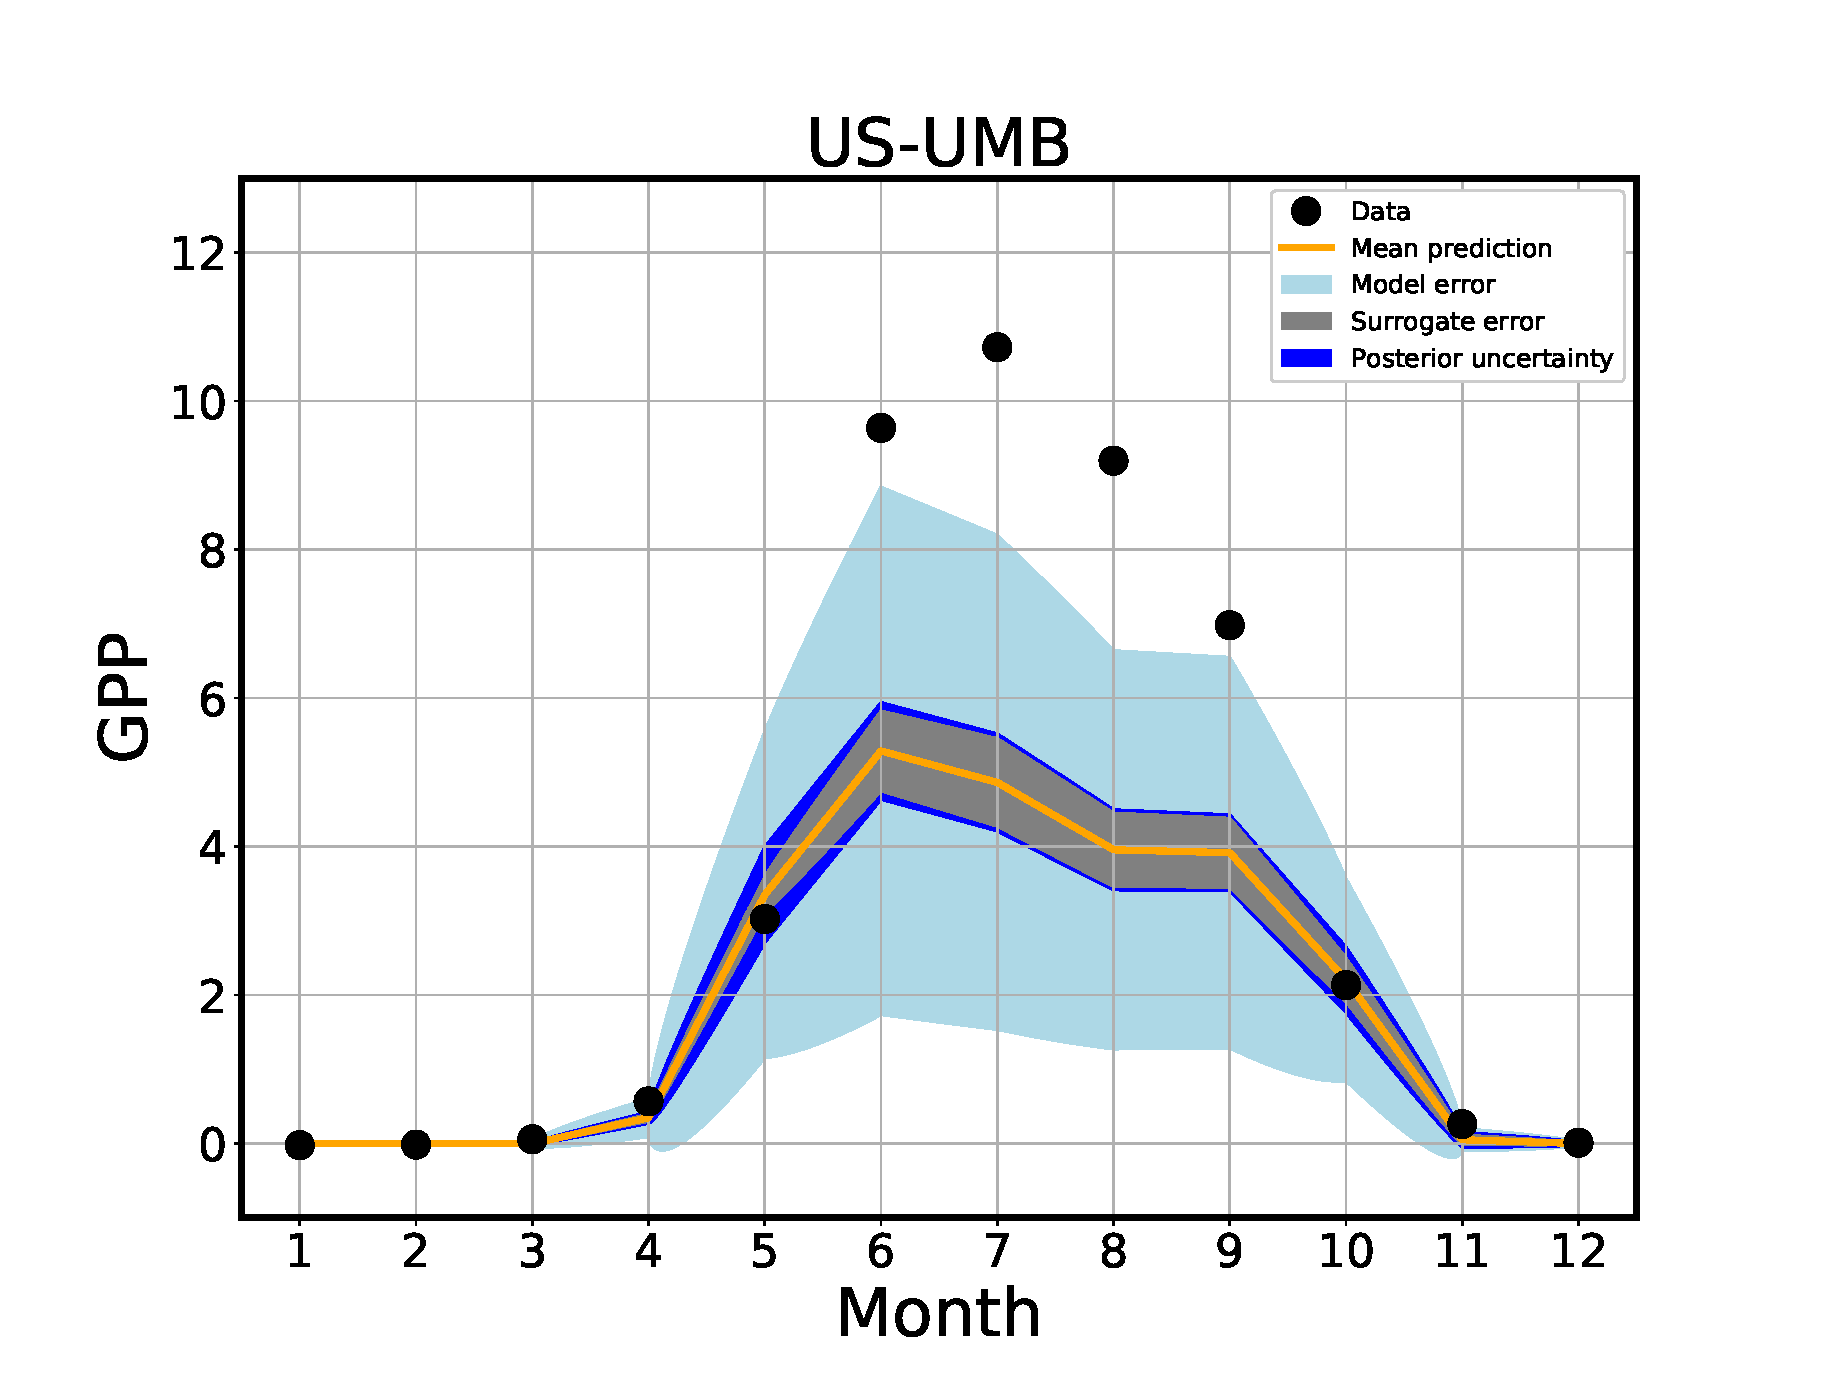
\includegraphics[width=0.24\textwidth]{figs_local/fit_US-UMB_merr.eps}
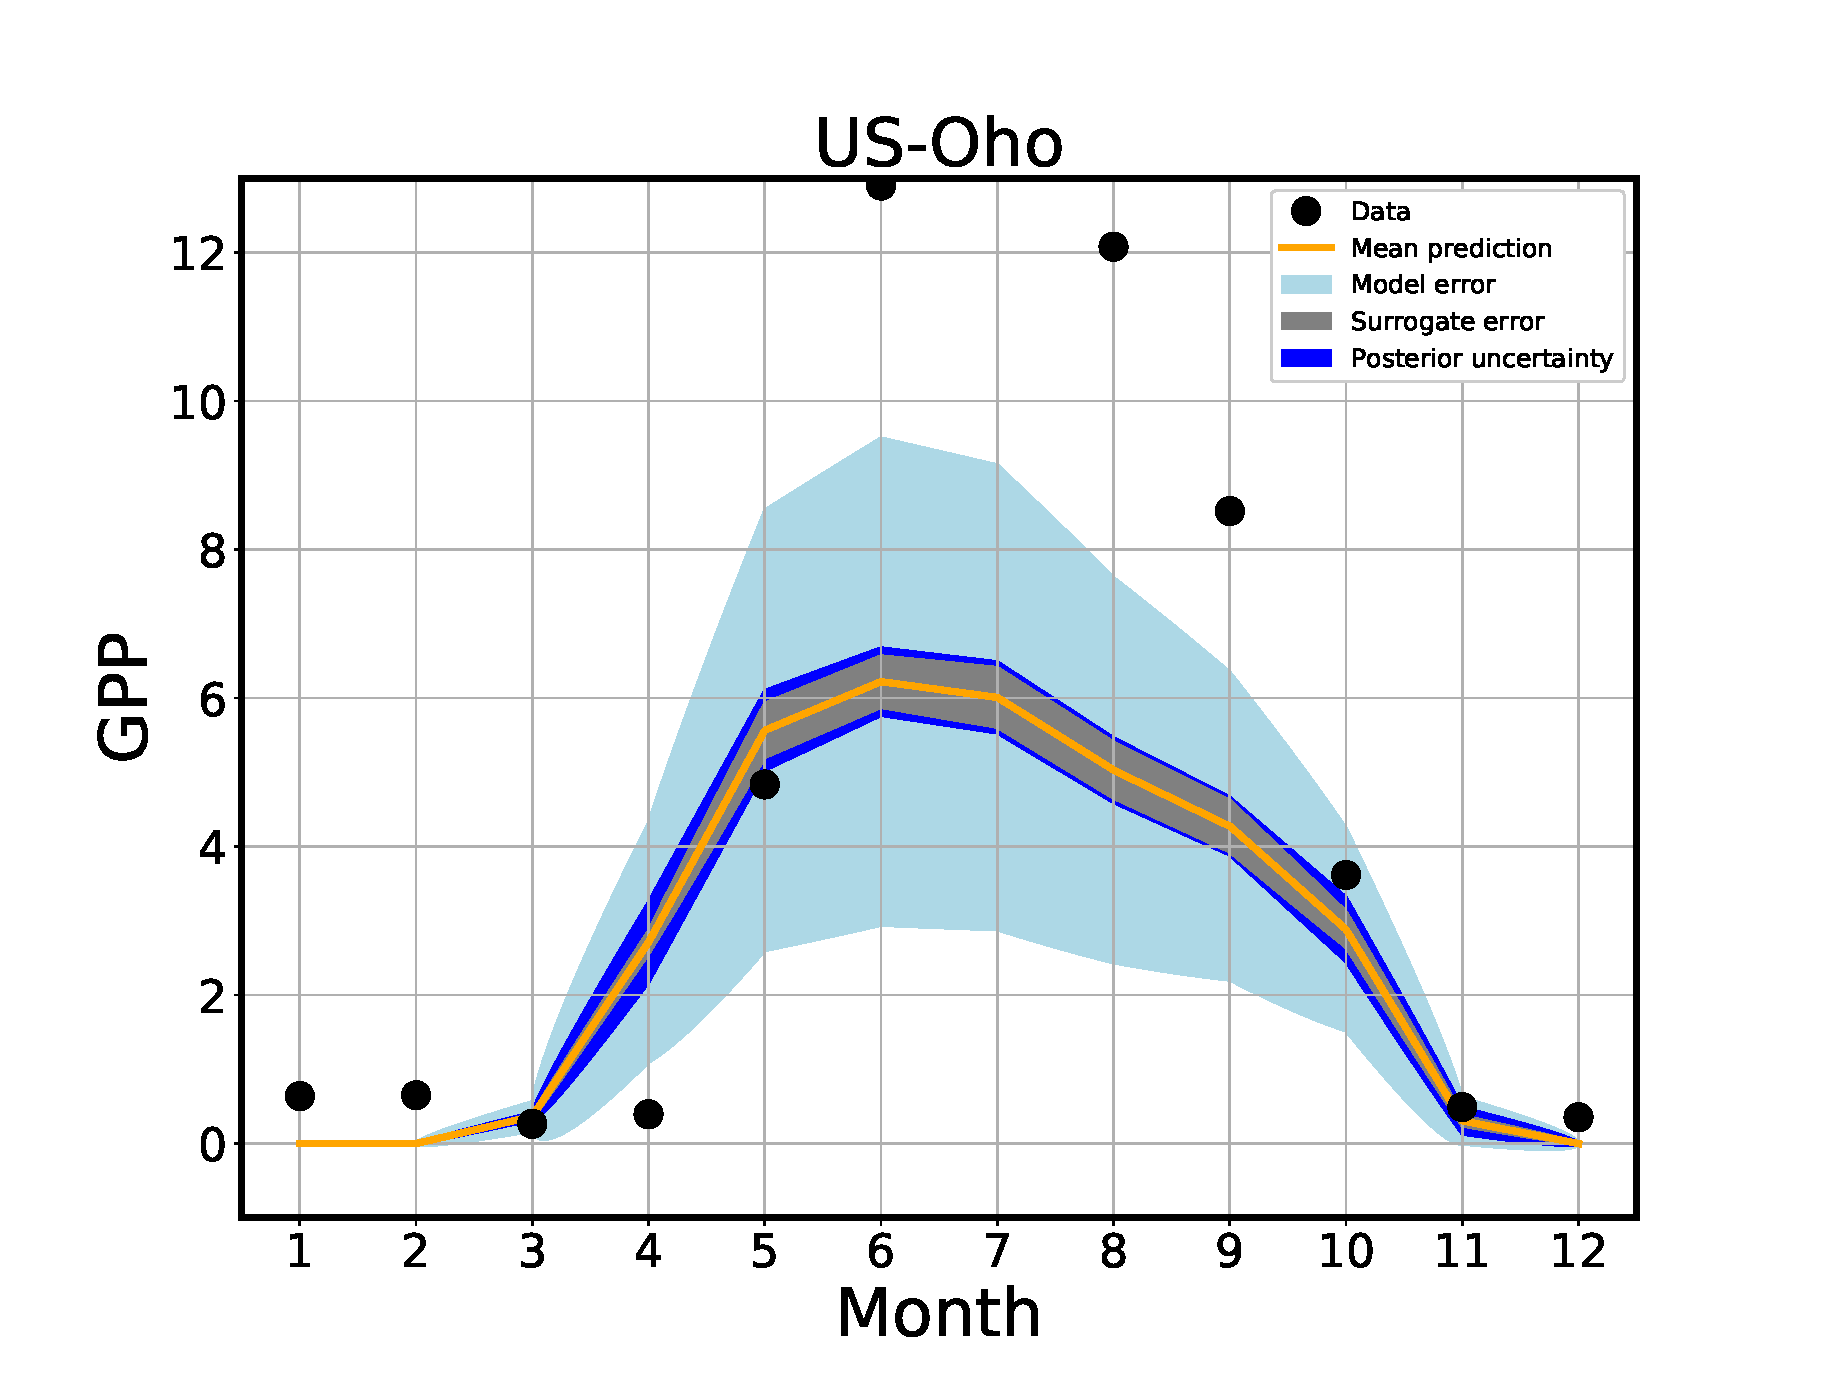
\includegraphics[width=0.24\textwidth]{figs_local/fit_US-Oho_merr.eps}
\end{center}
\bigskip
\hrule
\hrule
\bigskip
\medskip
\vspace*{0.5cm}

\fontsize{29}{29}\selectfont
 \textbf{Reference:} K. Sargsyan, X. Huan, H. Najm, Embedded model error representation for Bayesian model calibration, arXiv preprint arXiv:1801.06768, 2018.



\end{minipage}
};
\node[fancytitle, right=10pt, font=\fontsize{\fntszL}{\fntszL}\selectfont]
at (boxApp.north west) {\bf Application: E3SM Land Model};
